%##################################################################################################

\chapter{Performance of PLASMA}

\section{A Library for Multicore Architectures}

To achieve high performance on multicore architectures, \PLASMA
relies on tile algorithms, which provide fine granularity
parallelism. The standard linear algebra algorithms can then be
represented as Directed Acyclic Graphs (DAG) where nodes represent
tasks and edges represent dependencies among them.  Our programming
model enforces asynchronous, out of order scheduling of
operations. This concept is used as the basis for a scalable yet
highly efficient software framework for computational linear algebra
applications.

In \LAPACK, parallelism is obtained though the use of multithreaded
{\em Basic Linear Algebra Subprograms}~(\BLAS). In \PLASMA, parallelism is
no longer hidden inside the BLAS but is brought to the fore to yield
much better performance.

PLASMA performance strongly depends on tunable execution parameters
trading off utilization of different system resources.  The outer
block size (NB) trades off parallelization granularity and scheduling
flexibility with single core utilization, while the inner block size
(IB) trades off memory load with extra-flops.

\PLASMA is currently scheduled statically with a trade off between load
balancing and data reuse.

\section{Comparison to other libraries}
\label{sec:comparison}


We present here the performance of the three following one sided
factorizations: Cholesky, QR, and LU. We compare \PLASMA against
the two established linear algebra packages \LAPACK and \SCALAPACK. The
experiments were conducted on two different multicore architectures
based on Intel Xeon EMT64 and IBM Power6.

\PLASMA, \LAPACK and \SCALAPACK are all linked with the optimized
vendor \BLAS available on the system provided within Intel \MKL 10.1
and IBM \ESSL 4.3 on the \Intel and \Power architectures,
respectively. The first architecture is a quad-socket quad-core
machine based on an Intel Xeon EMT64 E7340 processor operating at
$2.39$ GHz. Its theoretical peak is equal to $9.6$ Gflop/s/ per core
or $153.2$ Gflop/s for the whole node (16 cores). The second
architecture is a SMP node composed of 16 dual-core Power6
processors. Each dual-core Power6 processor runs at $4.7$ GHz, leading
to a theoretical peak of $18.8$ Gflop/s per core and $601.6$ Gflop/s
per node (32 cores).

%\section{Methodology}
%\label{sec:comparison-methodology}

We only report double precision performance numbers for simplicity purposes.
\PLASMA is tuned
with the pruned search method as described in \cite{Agullo:2009:CS1}. For
\SCALAPACK, we have tuned the data distribution parameters (p,q,nb) as
functions of the number of cores and the matrix size through an
exhaustive search.  For reference LAPACK, we have been using the
default block size (no tuning).

\ignore{
Furthermore, to capture the best possible behavior of each library, we
repeat the number of executions (up to 10 times) and we report the
highest performance obtained. We do not flush the caches before timing
a factorization\footnote{It is kernel usage, not problem size, that
  dictates whether one wish to flush the cache. Warm (or partially
  warm) cache executions are plausible for dense linear
  factorizations. For instance, sparse linear solvers, which rely on
  dense kernels, intend to maximize data reuse between successive
  calls to dense operations.}. However, the TLB (Translation Lookaside
Buffer) is flushed between two executions: the loop over the different
executions is performed in a script (rather than within the
executable) and calls several times the same executable.
}

\SCALAPACK and \PLASMA interfaces allow the user to provide data
distributed on the cores. In our shared-memory multicore environment,
because we do not flush the caches, these libraries have thus the
advantage to start the factorization with part of the data distributed
on the caches. This is not negligible. For instance, a
$8000\times8000$ double precision matrix can be held distributed on
the L3 caches of the 32 cores of a \Power node.

%\subsection{Experimental results}

Figures~\ref{fig:ch}, \ref{fig:qr}, \ref{fig:lu} present performance
for the Cholesky, QR and LU factorizations, respectively.

\begin{figure}[htbp]
    \subfigure[Intel Xeon - 16 cores]{
      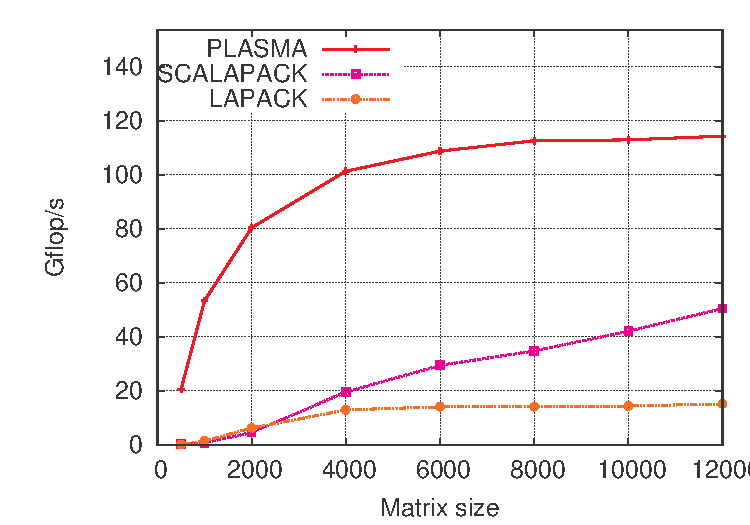
\includegraphics[width=\figwidth]{fig/Intel64-DPOTRF-PLASMA_SCALAPACK_LAPACK-16cores-short}
    }%
    \subfigure[Power6 - 32 cores]{
      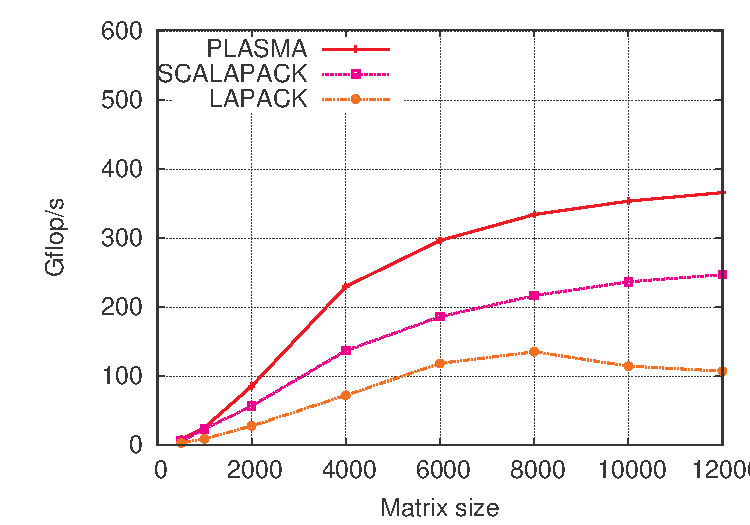
\includegraphics[width=\figwidth]{fig/Power6-DPOTRF-PLASMA_SCALAPACK_LAPACK-32cores-short}
    }%
  \caption{Performance of the Cholesky factorization (Gflop/s).}
  \label{fig:ch}
\end{figure}

\begin{figure}[htbp]
    \subfigure[Intel Xeon - 16 cores]{
      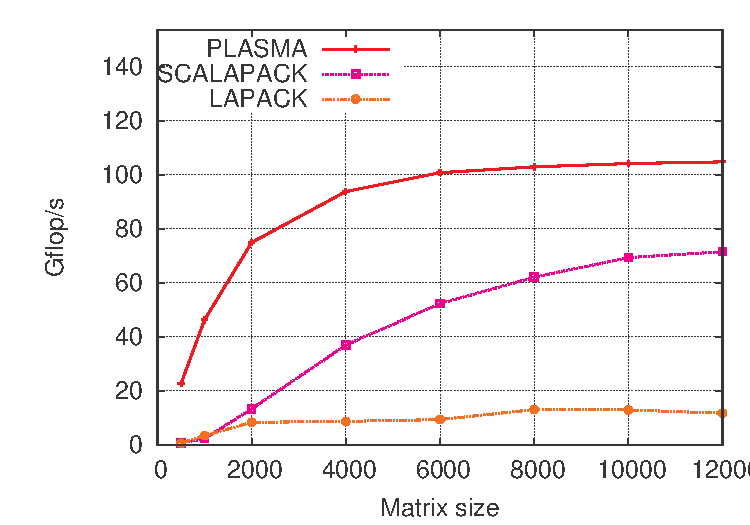
\includegraphics[width=\figwidth]{fig/Intel64-DGEQRF-PLASMA_SCALAPACK_LAPACK-16cores-short}
    }%
    \subfigure[Power6 - 32 cores]{
      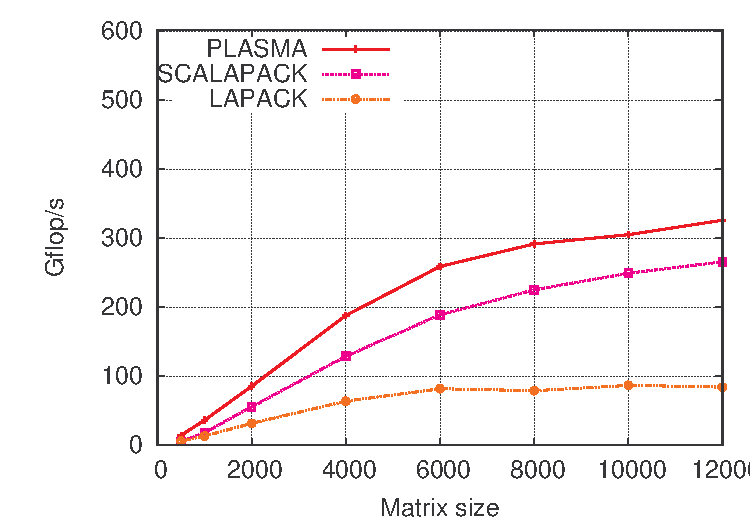
\includegraphics[width=\figwidth]{fig/Power6-DGEQRF-PLASMA_SCALAPACK_LAPACK-32cores-short}
    }%
  \caption{Performance of the QR factorization (Gflop/s).}
  \label{fig:qr}
\end{figure}

\begin{figure}[htbp]
    \subfigure[Intel Xeon - 16 cores]{
      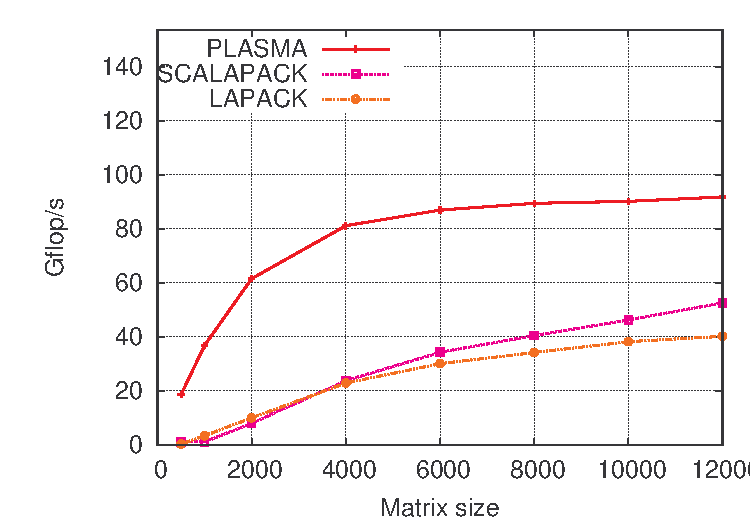
\includegraphics[width=\figwidth]{fig/Intel64-DGETRF-PLASMA_SCALAPACK_LAPACK-16cores-short}
    }%
    \subfigure[Power6 - 32 cores]{
      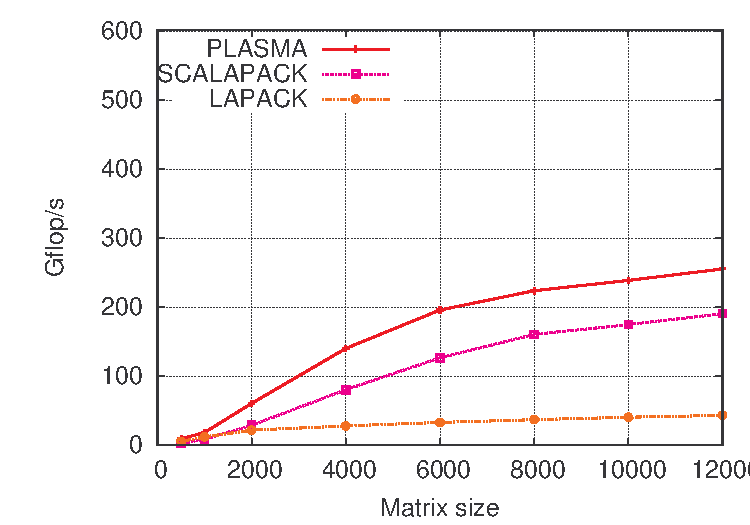
\includegraphics[width=\figwidth]{fig/Power6-DGETRF-PLASMA_SCALAPACK_LAPACK-32cores-short}
    }%
  \caption{Performance of the LU factorization (Gflop/s).}
  \label{fig:lu}
\end{figure}

\section{Tuning - Howto}

Users willing to obtain good performance from PLASMA need to tune PLASMA
parameters.  The example code below illustrates how to change the \texttt{NB}
and \texttt{IB} parameters before calling the appropriate PLASMA routine to
factorize or solve a linear system.

We recall that QR and LU algorithms requires both NB and IB parameters while Cholesky needs only NB.


\begin{verbatim}
...
       /* Plasma Tune */
       PLASMA_Disable(PLASMA_AUTOTUNING);
       PLASMA_Set(PLASMA_TILE_SIZE, NB);
       PLASMA_Set(PLASMA_INNER_BLOCK_SIZE, IB);
...
\end{verbatim}


A pruned search method to obtain ``good''
parameters is described in \cite{Agullo:2009:CS1}.  We note that autotuning is
part of the PLASMA's roadmap; unfortunately, as of 2.0.0, the PLASMA software
does not have its autotuning component available for release.

%###################################################################################################
